%\section{「印刷する」機能}
印刷する機能はユーザがカードリストから使用したい写真を選択することで、1枚のリーフレットを自動で作成する機能である。本機能は、写真選択画面、リーフレット作成画面、印刷プレビュー画面、AirPrintの設定画面の4つの画面から成り立つ。\\ 
ユーザが最初に見る画面は写真選択画面である。この画面へはトップ画面の「印刷する」ボタンをタップすることで遷移する。遷移したときの画面を図6.7(a)に示す。この画面はリーフレットと縦横比が同一になっており、横スクロールすることでリーフレットの全体を見ることができる。リーフレットの詳細については6章5節を参照されたい。また、写真撮影画面内に表示している「タップして写真をえらぶ」と書かれている枠内をタップするとリーフレット作成画面に遷移する。このときの画面を図6.7(b)に示す。リーフレット作成画面ではリーフレットで使いたい写真をユーザに選んでもらう。表示された写真の中にユーザが使用したい写真があれば「この写真を使う」ボタンをタップすることで写真選択画面に遷移し、「タップして写真をえらぶ」と書かれている枠内が選択した写真に変更される。このようにしてリーフレットに使いたい写真を7枚選んでもらう。リーフレットに使う写真が7枚であるため、7枚選んでいない状態で写真選択画面の右上に表示している「完了」ボタンをタップすると警告が表示される。警告は全ての枠に対して写真を選択するように注意する内容である。ユーザが7枚全てを選んだ状態で「完了」ボタンをタップすると印刷プレビュー画面に遷移する。このときの画面を図6.7(c)に示す。印刷プレビュー画面では、リーフレットの表側、裏側がどのように印刷されるのかを確認することができる。もし、印刷されるリーフレットを修正したい場合は左上の「戻る」ボタンをタップして写真選択画面に戻ることができる。印刷プレビューに表示しているリーフレットを印刷する場合は右上の「印刷」ボタンを押すことでAirPrint\footnote{AirPrintはApple Inc.の商標}の設定画面に遷移する。このときの画面を図6.6(d)に示す。AirPrintの設定画面ではまず、接続するプリンタを選択する。iPhoneとプリンタがWi-Fiに接続されている場合はプリンタの欄に使用可能なプリンタ名が表示される。次に、印刷する部数および印刷するページを片面か両面かを選択した後、右上の「プリント」ボタンをタップするとiPhoneからプリンタにデータが送信される。そして、プリンタがWi-Fi経由でデータを受信するとリーフレットが印刷される。
\begin{figure}[htbp]
  \begin{center}
    \begin{tabular}{c}

      % 1
      \begin{minipage}{0.33\hsize}
        \begin{center}
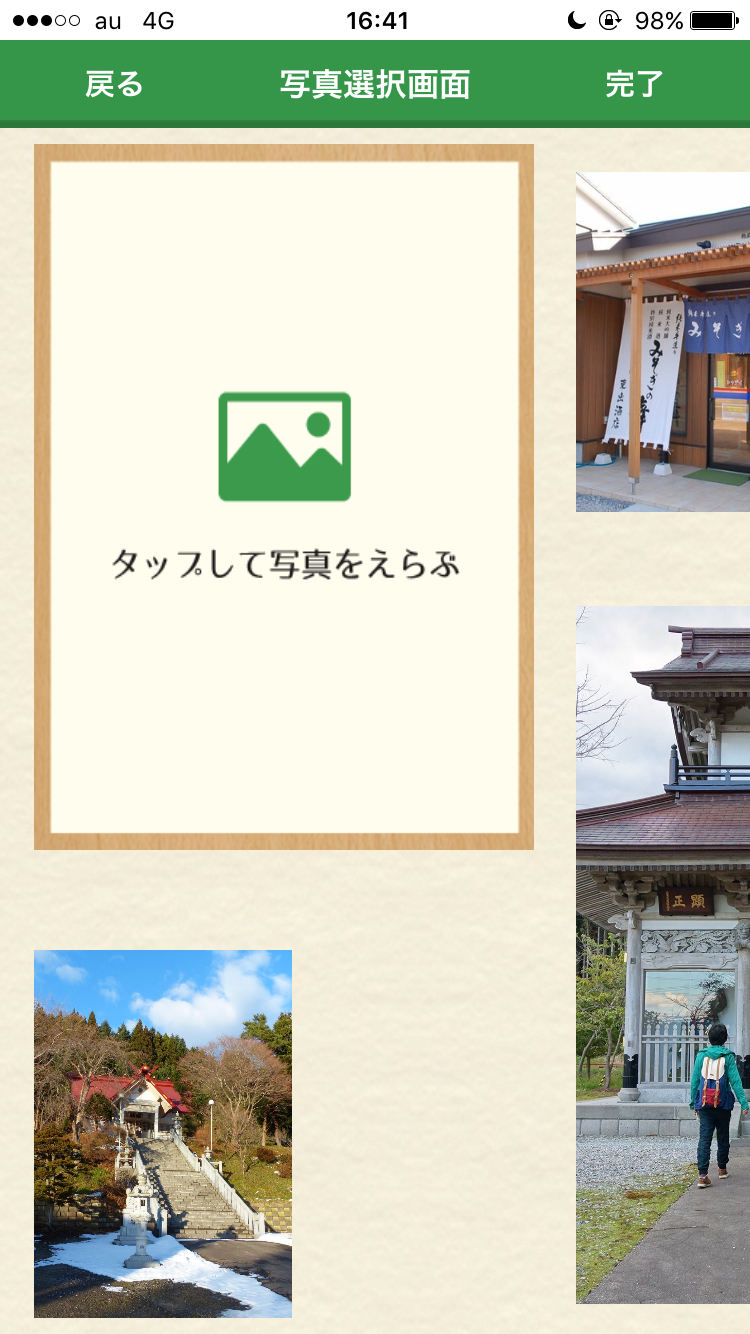
\includegraphics[width=4cm, bb=0 0 304 570]{kiko_print2.PNG}
          \hspace{1cm} (a)写真選択画面
        \end{center}
      \end{minipage}

      % 2
      \begin{minipage}{0.33\hsize}
        \begin{center}
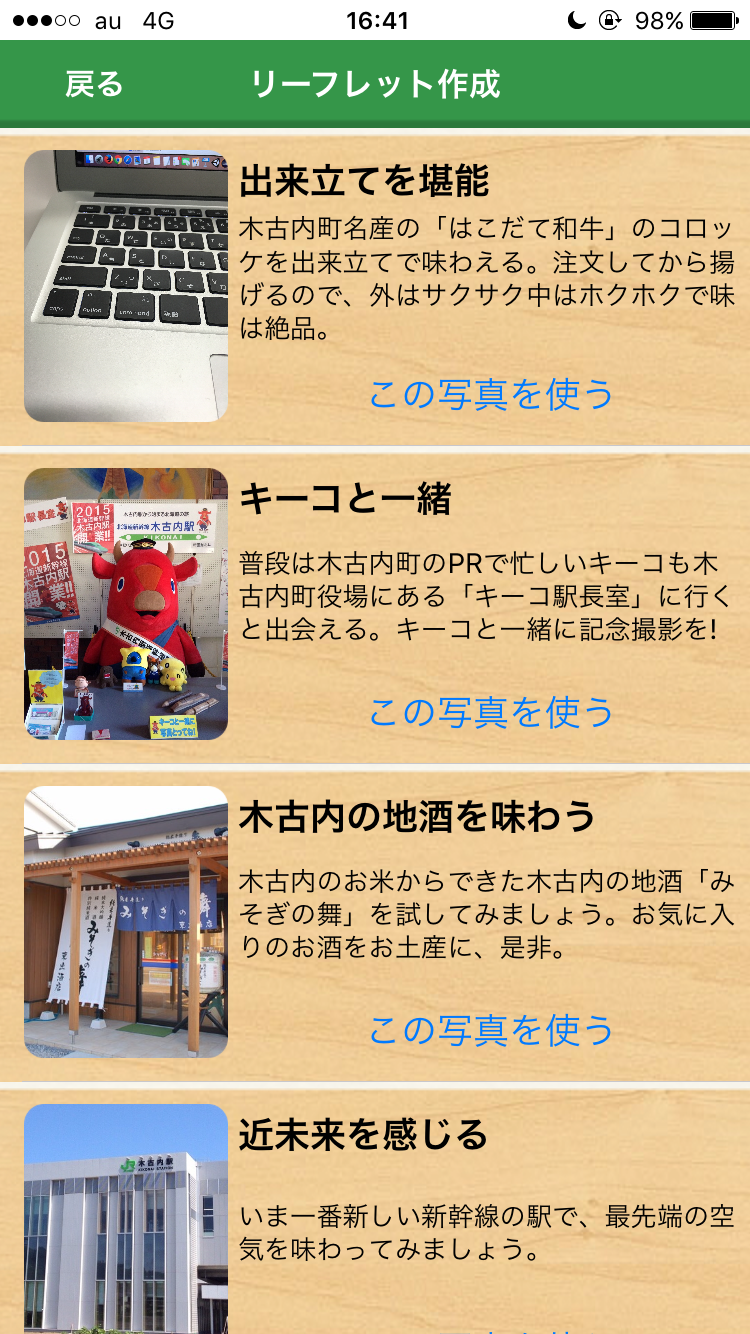
\includegraphics[width=4cm, bb=0 0 304 570]{kiko_print3.PNG}
          \hspace{1cm} (b)リーフレット作成画面
        \end{center}
      \end{minipage}
      
      \\
      
       % 3
      \begin{minipage}{0.33\hsize}
        \begin{center}
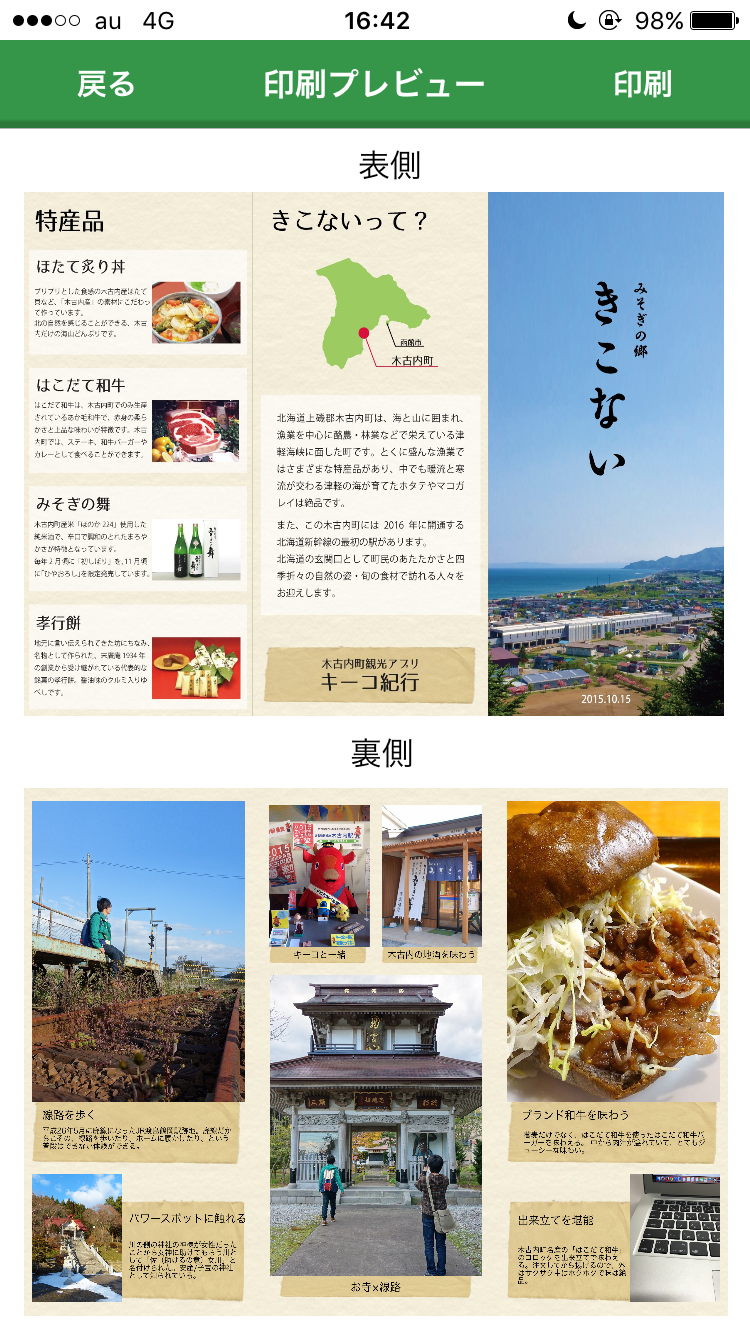
\includegraphics[width=4cm, bb=0 0 304 570]{kiko_print4.PNG}
          \hspace{1cm} (c)印刷プレビュー画面
        \end{center}
      \end{minipage}

      % 4
      \begin{minipage}{0.33\hsize}
        \begin{center}
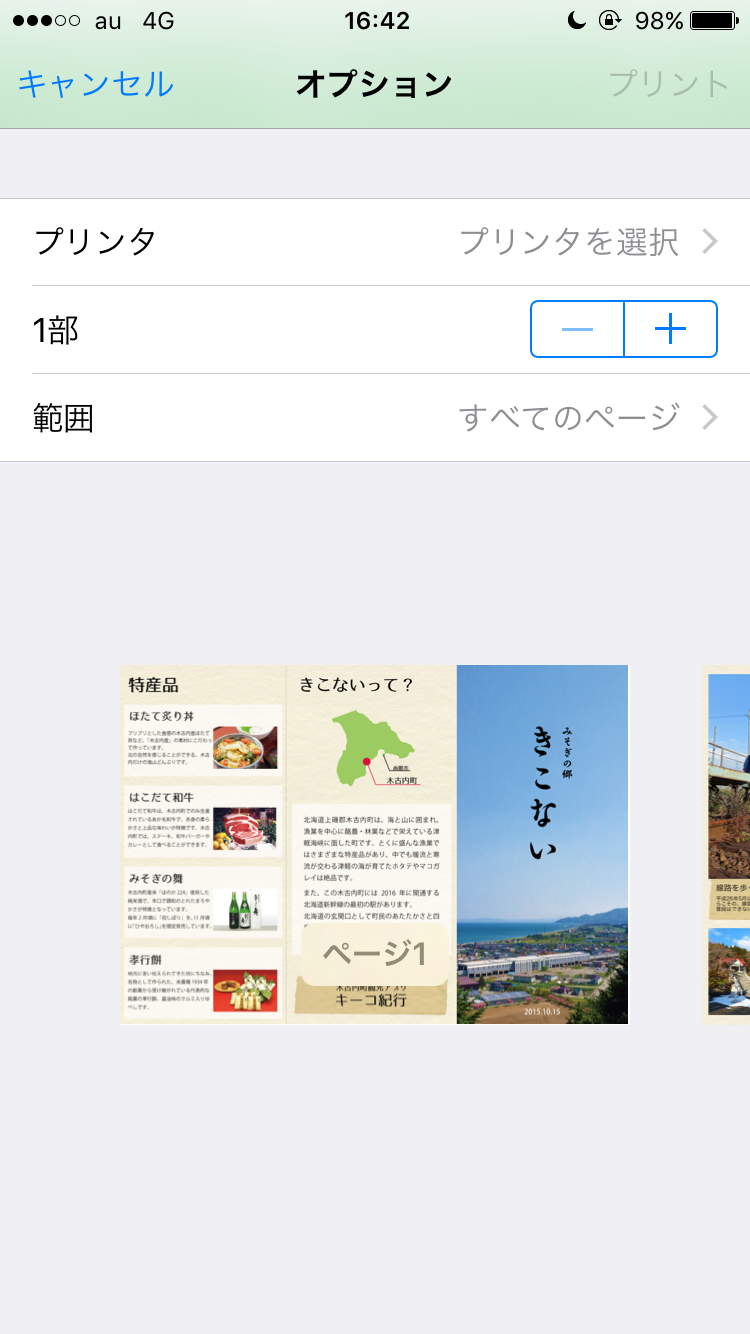
\includegraphics[width=4cm, bb=0 0 304 570]{kiko_print5.PNG}
          \hspace{1cm} (d)AirPrintの設定画面
        \end{center}
      \end{minipage}
      

    \end{tabular}
    \caption{印刷機能の画面}
    \label{fig:lena}
  \end{center}
\end{figure}       

\bunseki{池田俊輝}